\documentclass[11pt]{article}

\usepackage{fullpage}% reasonable margins
\usepackage{array} % makes tables nicer
\usepackage{comment} %block comments
\usepackage{color} %colored text
\usepackage{graphicx} %images


%squeezed itemize for table.
\newenvironment{packed_itemize}{
\begin{itemize}
  \setlength{\itemsep}{1pt}
  \setlength{\parskip}{0pt}
  \setlength{\parsep}{0pt}
}{\end{itemize}}

\title{\bf YAExS Stakeholder Review 1}
\author{TimeFinders: Andrew Karnani, Auston Sterling, Jeffrey Rodowicz, Vera Axelrod}
\date{October 29, 2012}

\begin{document}
\maketitle
\hrule
\vspace{0.03in}
\hrule
%%%%%%%%%%%%%%%%%%%%%%%%%%
%%%%%%%%%%%%%%%%%%%%%%%%%%
%\section*{Demonstration} % ANDREW + AUSTON %
%%%%%%%%%%%%%%%%%%%%%%%%%%
% DONT NEED TO WRITE ANYTHING

%%%%%%%%%%%%%%%%%%%%%%%%%%
%%%%%%%%%%%%%%%%%%%%%%%%%%
\section{Sequence Diagrams} % VERA %
%%%%%%%%%%%%%%%%%%%%%%%%%%
\begin{comment}
\textcolor{red}{
Interaction diagrams showing how a specific Use Case is realized within the beta version of the software. The diagrams must use correct UML notation.  Check for proper UML, and makes sense.}
\end{comment}

A sequence diagram for the log-in use case is shown in figure \ref{fig:logInSeq}
 while figure \ref{fig:startSeq} shows a sequence diagram for the start scheduling 
use case.  We have also included a sequence diagram for the ``could" implement feature view schedule, shown in figure \ref{fig:viewSeq}. 

\begin{figure}
	\centering
		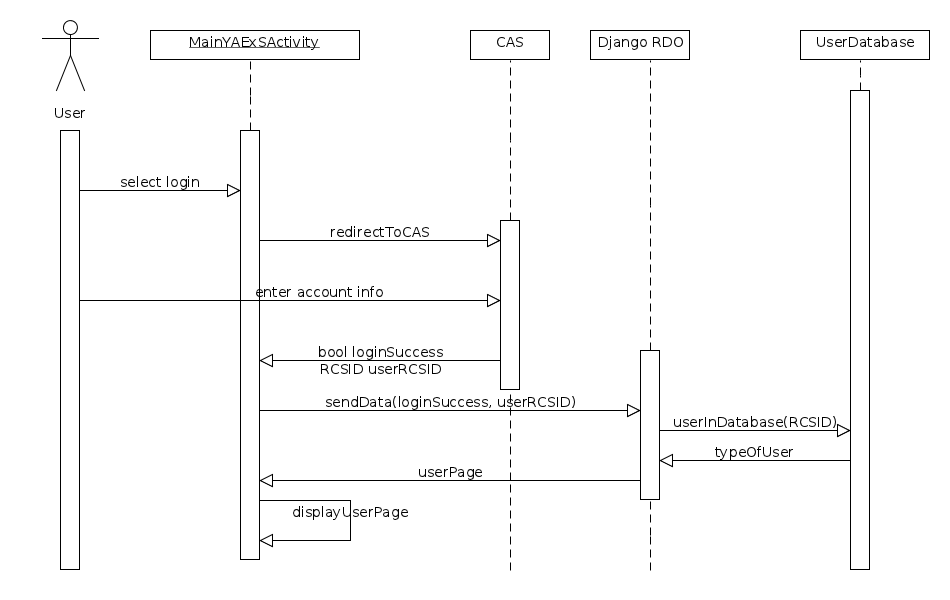
\includegraphics[width = 0.9\textwidth]{logInSequence.png}
	\caption{\textbf{Log-In Sequence Diagram}}
	\label{fig:logInSeq}
%\end{figure}
\vspace{0.4in}
%\begin{figure}
%	\centering
		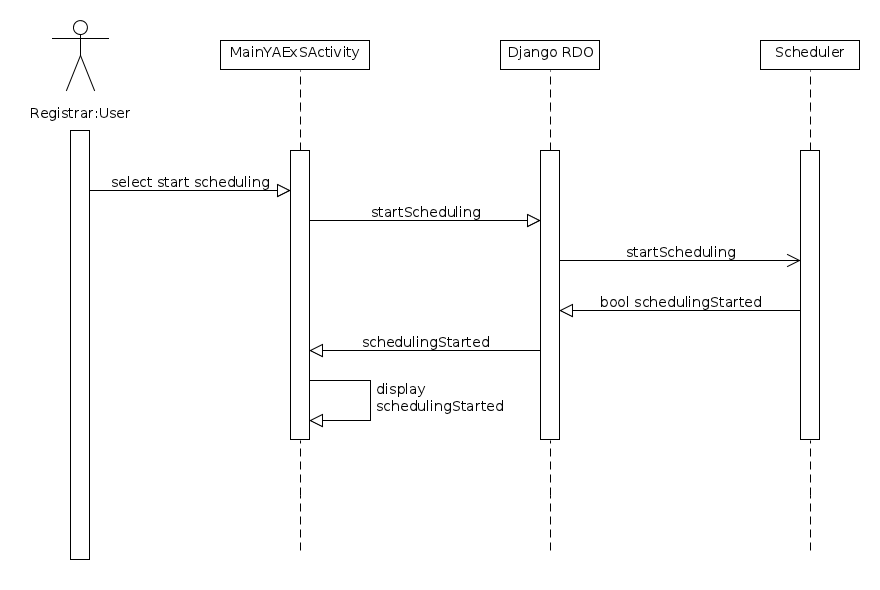
\includegraphics[width = .9\textwidth]{startSchedulingSequence.png}
	\caption{\bf Start Scheduling Sequence Diagram}
	\label{fig:startSeq}
\end{figure}


\begin{figure}
	\centering
		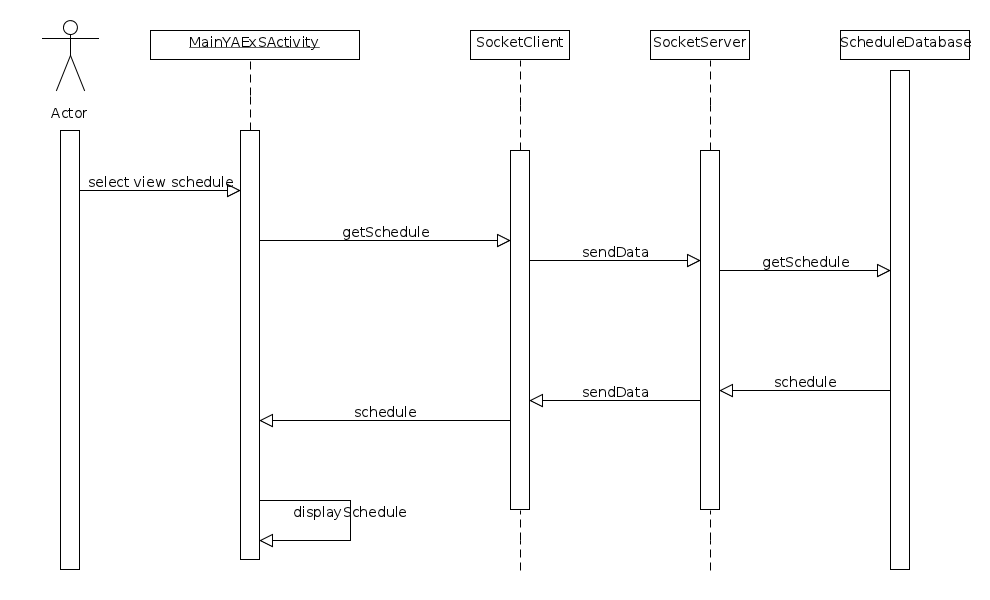
\includegraphics[width = \textwidth]{viewScheduleSequence.png}
	\caption{\bf View Schedule Sequence Diagram}
	\label{fig:viewSeq}
\end{figure}



%%%%%%%%%%%%%%%%%%%%%%%%%%
%%%%%%%%%%%%%%%%%%%%%%%%%%
\section{Static Class Diagram}  % JEFF %
%%%%%%%%%%%%%%%%%%%%%%%%%%
%\textcolor{red}{A static class diagram of the project's internal software structure. The diagram must be valid UML and accurately depict the software.  Check for proper UML, and makes sense.}
Our static class diagram is shown in figure \ref{fig:staticDiagram}.

% @JEFF: Simply uncomment the \includegraphics line below, change the name of the graphics file to be the static class diagram file you made.
\begin{figure}
	\centering
%		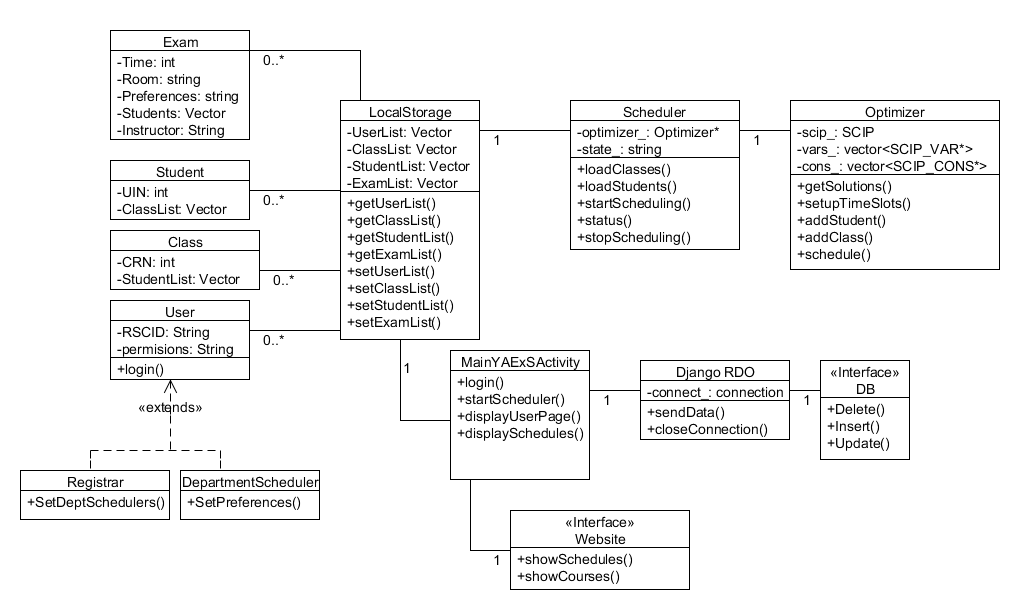
\includegraphics[width = \textwidth]{staticClassDiagram.png}
	\caption{\bf Static Class Diagram}
	\label{fig:staticDiagram}
\end{figure}


%%%%%%%%%%%%%%%%%%%%%%%%%%
%%%%%%%%%%%%%%%%%%%%%%%%%%
\section{ Design Approach}  % JEFF? %
%%%%%%%%%%%%%%%%%%%%%%%%%%

Our team broke our project into two main sections: 1) our website, including our database, and 2) the scheduler itself. The main design pattern that we are implementing will be the 
Model–-view–-controller  % you need double dashes to show the hyphens
pattern. Our model is the database and the final exam schedule, the view is what the website shows to the end user, and the controller is the user interface of the website . 

 We have also created a Postgres database that will store all of our data centrally, and are we are working on creating a standard for the data.  The standard will depend on the data that we are able to obtain from the Registrar.  We have also created a framework for communication between the website and database and SCIP, our schedule solver. This will use the mediator design pattern to handle the interaction. 

Both our website and our scheduling program are being designed in a modular way, which will enable us to implement one piece at a time and is conducive to the iterative approach that we are taking.


%%%%%%%%%%%%%%%%%%%%%%%%%%
%%%%%%%%%%%%%%%%%%%%%%%%%%
\section{Contribution Summary} % ALL %
%%%%%%%%%%%%%%%%%%%%%%%%%%
\begin{tabular}{|m{1.4in}|m{4.4in}|}
\hline 
\textbf{\large Name}     & \textbf{\large Contributions} \\
\hline\hline

 Andrew Karnani
	&
	 \begin{packed_itemize}
		\item Created Database Skeleton
		\item Designed Website User Interface Prototypes
		\item Tested CAS Authentication
	\end{packed_itemize}
\\
\hline
 Auston Sterling
	&
	 \begin{packed_itemize}
	        \item Created Scheduler Code Skeleton
		  \item Set Up SCIP
	\end{packed_itemize}
\\
\hline
Jeffrey Rodowicz
	&
	 \begin{packed_itemize}
		\item Created Static Class Diagram
		\item Wrote Design Approach
	\end{packed_itemize}
\\
\hline
Vera Axelrod
	&
	 \begin{packed_itemize}
		\item Created Sequence Diagrams
		\item Assisted in Design of Website User Interface Prototypes
		\item Wrote Contribution Summary
		\item Updated Status Report
	\end{packed_itemize}
\\
\hline
\end{tabular}

%%%%%%%%%%%%%%%%%%%%%%%%%%
%%%%%%%%%%%%%%%%%%%%%%%%%%
\section{Status Report} % VERA %
%%%%%%%%%%%%%%%%%%%%%%%%%%
\subsection{Things We've Done}
\begin{itemize}
	\item Created static class diagrams.
	\item Created sequence diagrams.
	\item Implemented a demonstration of the department scheduler web interface.
	\item Set up SCIP and all dependencies.
	\item Starting drafting an optimization model. 
\end{itemize}

\subsection{Challenges}
\begin{itemize}
	\item Delays in obtaining data from RPI Administration may cause future delays in our delivery.
	\item Need to set up and test a server for our program. The RPI Administration has not yet made it clear whether we will be able to run our program on an official RPI server in the future.
	\item Supporting older versions of Internet Explorer.
\end{itemize}

\subsection{Upcoming Plans}
\begin{itemize}
	\item Learn about warm starting the scheduling in SCIP.
	\item Fully define data formats with Registrar.
	\item Develop a way to detect and handle cross-referenced courses.
	\item Design and implement an algorithm to assign rooms to scheduled exams.
	\item Create an interface to display exam schedules. 
	\item Write object calisthenics sample code.
\end{itemize}

\end{document}